
\documentclass[12pt]{article}

% Layout.
\usepackage[top=1in, bottom=0.75in, left=1in, right=1in, headheight=1in, headsep=6pt]{geometry}

% Fonts.
\usepackage{mathptmx}
\usepackage[scaled=0.86]{helvet}
\renewcommand{\emph}[1]{\textsf{\textbf{#1}}}

% TiKZ.
\usepackage{tikz, pgfplots}
\usetikzlibrary{calc,trees,positioning,arrows,fit,shapes,calc}
\pgfplotsset{compat = newest}
\tikzset{
  jumpdot/.style={mark=*,solid},
  excl/.append style={jumpdot,fill=white},
  incl/.append style={jumpdot,fill=black},
}
 
\pgfplotsset{my style/.append style={axis x line=middle, axis y line=
middle, xlabel={$x$}, ylabel={$y$}, axis equal }}


% Misc packages.
\usepackage{amsmath,amssymb,latexsym}
\usepackage{graphicx}
\usepackage{array}
\usepackage{xcolor}
\usepackage{multicol}

% Commands to set various header/footer components.
\makeatletter
\def\doctitle#1{\gdef\@doctitle{#1}}
\doctitle{Use {\tt\textbackslash doctitle\{MY LABEL\}}.}
\def\docdate#1{\gdef\@docdate{#1}}
\docdate{Use {\tt\textbackslash docdate\{MY DATE\}}.}
\def\doccourse#1{\gdef\@doccourse{#1}}
\let\@doccourse\@empty
\def\docscoring#1{\gdef\@docscoring{#1}}
\let\@docscoring\@empty
\def\docversion#1{\gdef\@docversion{#1}}
\let\@docversion\@empty
\makeatother

% Headers and footers layout.
\makeatletter
\usepackage{fancyhdr}
\pagestyle{fancy}
\fancyhf{} % Clears all headers/footers.
\lhead{\baselineskip 30pt
%\emph{\@doctitle\hfill\@docdate}
\emph{\@docdate\hfill\@doctitle}
\ifnum \value{page} > 1\relax\else\\
\emph{Name: \rule{3.5in}{1pt}\hfill \@docscoring}\fi}
\rfoot{\emph{\@docversion}}
\lfoot{\emph{\@doccourse}}
\cfoot{\emph{\thepage}}
\renewcommand{\headrulewidth}{0pt}%
\makeatother

% Paragraph spacing
\parindent 0pt
\parskip 6pt plus 1pt

% A problem is a section-like command. Use \problem{5} to
% start a problem worth 5 points.
\newcounter{probcount}
\newcounter{subprobcount}
\setcounter{probcount}{0}
\newcommand{\problem}[1]{%
\par
\addvspace{4pt}%
\setcounter{subprobcount}{0}%
\stepcounter{probcount}%
%\makebox[0pt][r]{\emph{\arabic{probcount}.}\hskip1ex}\emph{[#1 points]}\hskip1ex}
\makebox[0pt][r]{\emph{\arabic{probcount}.}\hskip1ex}\emph{[#1 \ifnum1=0#1\relax point\else points\fi]}\hskip1ex}
%\textbf{(#1 \ifnum1=0#1\relax thing\else things\fi
\newcommand{\thesubproblem}{\emph{\alph{subprobcount}.}}

% Subproblems are an enumerate-like environment with a consistent
% numbering scheme. 
% Use \begin{subproblems}\item...\item...\end{subproblems}
\newenvironment{subproblems}{%
\begin{enumerate}%
\setcounter{enumi}{\value{subprobcount}}%
\renewcommand{\theenumi}{\emph{\alph{enumi}}}}%
{\setcounter{subprobcount}{\value{enumi}}\end{enumerate}}

% Blanks for answers in normal and math mode.
\newcommand{\blank}[1]{\rule{#1}{0.75pt}}
\newcommand{\mblank}[1]{\underline{\hspace{#1}}}
\def\emptybox(#1,#2){\framebox{\parbox[c][#2]{#1}{\rule{0pt}{0pt}}}}

% Misc.
\renewcommand{\d}{\displaystyle}
\newcommand{\ds}{\displaystyle}
\def\bc{\begin{center}}
\def\ec{\end{center}}
\def\be{\begin{enumerate}}
\def\ee{\end{enumerate}}

\newcommand{\ans}{\rule{2 in}{.5pt}}
\newcommand{\bigans}[1]{\rule{#1 in}{.5pt}}

\doctitle{Math F251X: Quiz 4}
\docdate{Fall 2026}
\doccourse{UAF Calculus I}
\docversion{v-1}
\docscoring{\blank{0.8in} / 25}
\begin{document}
\textbf{Please circle your section:} \hfill 901 (Gossell)  \hfill 902 (Gossell) \hfill 903 (Graves-McCleary)\\

No aids (book, calculator, etc.) are permitted.  {\bf Show all work for full credit.}

%Problem
\problem{8} Consider the function $\displaystyle f(x)=\frac{2}{3-x}$.\\

Find $f'(1)$ using the limit definition: $\displaystyle f'(x)=\lim_{h \rightarrow 0}\frac{f(x+h)-f(x)}{h}$.\\

(Finding the derivative using any other derivative method will result in 0 points for this problem.)
\vfill

$f'(1)=$\\

\problem{5} Using the graph of $g(x)$ below, sketch a graph of {\bf the derivative} $g'(x)$ on the axis to the right.

\begin{multicols}{2}

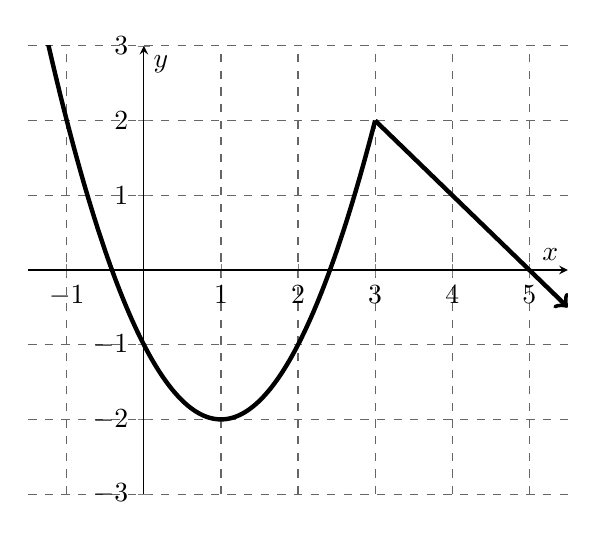
\begin{tikzpicture}[scale=1]
 \begin{axis}[
    xmin = -1.5, xmax = 5.5,
    ymin = -3, ymax = 3, xtick={-1,0,1,...,4,5}, ytick={-3,-2,...,3},
    grid=both, grid style={ thin, black!60, dashed},axis x line=middle, axis y line=
middle, xlabel={$x$}, ylabel={$y$}]
    \addplot[ultra thick, -,samples=200,
        domain = -2:3,
    ] {(x-1)^2-2};
    \addplot[ultra thick,->] coordinates {(3,2)(5.5,-0.5)};
\end{axis}
\end{tikzpicture}

\begin{tikzpicture}[scale=1]
 \begin{axis}[
    xmin = -1.5, xmax = 5.5,
    ymin = -3, ymax = 3, xtick={-1,0,1,...,4,5}, ytick style={draw=none},
yticklabels=\empty,
    %grid=both, grid style={ thin, black!60, dashed},
    axis x line=middle, axis y line=middle, xlabel={$x$}, ylabel={$y$}
]

\end{axis}
\end{tikzpicture}

\end{multicols}

\newpage

\problem{12} Find the derivative of each function. You may use any method you like, and you do not need to simplify your answer.
\begin{subproblems}
\item $\displaystyle f(x)=4x^7-5x^6+\frac{x}{6}-7$
\vfill
$f'(x)=$\\

\item $\displaystyle g(x)=\frac{30+x-x^4}{x^2}$
\vfill
$g'(x)=$\\

\item $\displaystyle h(x)=\cos(x)\left(x^4+x^3+x+1\right)$
\vfill
$h'(x)=$\\

\item $\displaystyle p(x)=\sqrt{x}\left(x^2+\cos(x)\right)+2^4$
\vfill
$p'(x)=$\\
\end{subproblems}



\end{document}
%%% Local Variables:
%%% mode: LaTeX
%%% TeX-master: t
%%% End:
